\documentclass[serif,xcolor=pdftex,dvipsnames,table,hyperref={bookmarks=false,breaklinks}]{beamer}

%%%%%%%%%%%%%%%%
% Change the macros below to configure the title slides
% for your course.
\newcommand{\coursename}{COMPSCI 589}
\newcommand{\instructor}{Benjamin M. Marlin}
\newcommand{\university}{University of Massachusetts Amherst}
\newcommand{\department}{College of Information and Computer Sciences}
%%%%%%%%%%%%%%%%


\newcommand{\settitlecard}[2]{
  \title[\coursename  Lecture #1] 
    {\coursename \\ Lecture #1: #2}
     \author[\instructor]{\instructor}
     \institute[\university]{
     \department\\
     \university
   }
\date{}
}

\newcommand{\maketitlepage}{
  \begin{frame}
  \titlepage
  \center{
    %If you use the slides unmodified, retain the attribution below
    \tiny{Slides by Benjamin M. Marlin (marlin@cs.umass.edu). \\
    \vspace{-1em}Created with support from National Science Foundation Award\# IIS-1350522. 
    %If you modify the slides, please retain the alternate attribution below
    %\tiny{Based on slides by Benjamin M. Marlin (marlin@cs.umass.edu). \\    
    %\vspace{-1em}Created with support from National Science Foundation Award\# IIS-1350522. 
    }                                              
  }  
  \end{frame}
}

\AtBeginSection[]
{
  \begin{frame}<beamer>{Outline}
    \tableofcontents[currentsection,subsectionstyle=hide]
  \end{frame}
}


\newcommand{\cut}[1]{}

\newcommand{\iconbox}[4]{
  \only<#1-#2>{
    \begin{columns}[T]
      \column{0.5in}
           \includegraphics[width=0.5in]{#3}
       \column{3.7in}
            #4
    \end{columns}
    \medskip
    \medskip
    \medskip
  }
}

\mode<presentation>{
  \usepackage{../beamertheme589theme}
  \setbeamercovered{invisible}
}

\mode<handout>{
  \usepackage{../beamertheme589theme}
  \setbeamercovered{transparent}
}


\usepackage[english]{babel}
\usepackage[latin1]{inputenc}
\usepackage{times}
\usepackage[T1]{fontenc}
\usepackage{amsmath}
\usepackage{amssymb}
\usepackage[noend]{algorithmic}
\usepackage{algorithm}
\usepackage{listings}

\renewcommand\mathfamilydefault{\rmdefault}

\newcommand{\setA}{\mathcal{A}}
\newcommand{\setB}{\mathcal{B}}
\newcommand{\setS}{\mathcal{S}}
\newcommand{\setV}{\mathcal{V}}
\DeclareMathOperator*{\union}{\bigcup}
\DeclareMathOperator*{\intersection}{\bigcap}
\DeclareMathOperator*{\Val}{Val}
\newcommand{\mbf}[1]{{\mathbf{#1}}}
\DeclareMathOperator*{\argmax}{arg\,max}
\DeclareMathOperator*{\argmin}{arg\,min}
\DeclareMathOperator*{\sign}{sign}
\newcommand{\deriv}[2]{\frac{\partial{#1}}{\partial{#2}}}


\settitlecard{12}{Introduction to Data Parallel Computing}

\begin{document}

\maketitlepage



\section{Parallel Hardware}
\subsection{foo}

\begin{frame}[t]{Moore's Law}
\center
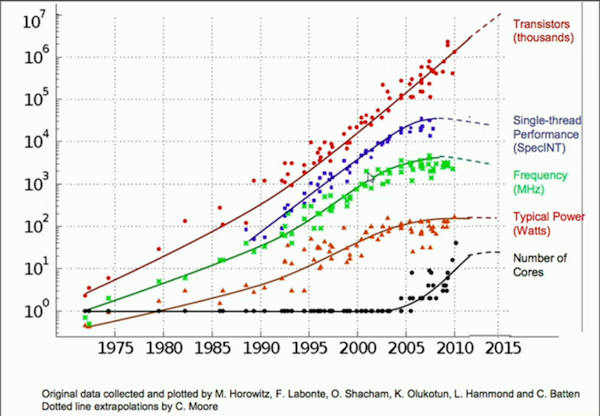
\includegraphics[width=3.5in]{../Figures/moores_law.png}\\[6pt]

\pause Machine Learning's free ride ended in about 2005.
\end{frame}

\begin{frame}[t]{Multi-Core CPUs}
\center
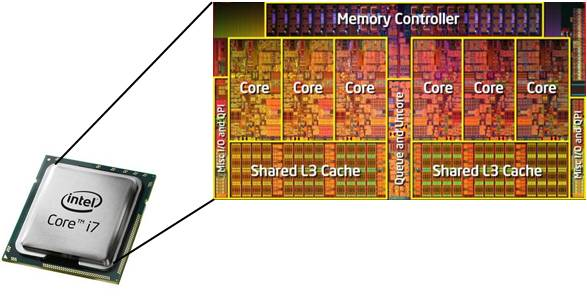
\includegraphics[width=4in]{../Figures/corei7.jpg}
\end{frame}

\begin{frame}[t]{Multi-Core CPU Memory Architecture}
\center
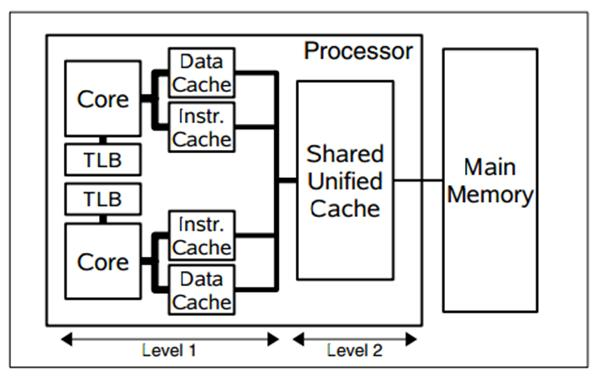
\includegraphics[width=3.5in]{../Figures/multi-core-architecture.jpg}\\[12pt]
\pause\textbf{Question:} What if one multi-core CPU isn't enough?
\end{frame}

\begin{frame}[t]{Distributed Computer (Cluster)}
\center
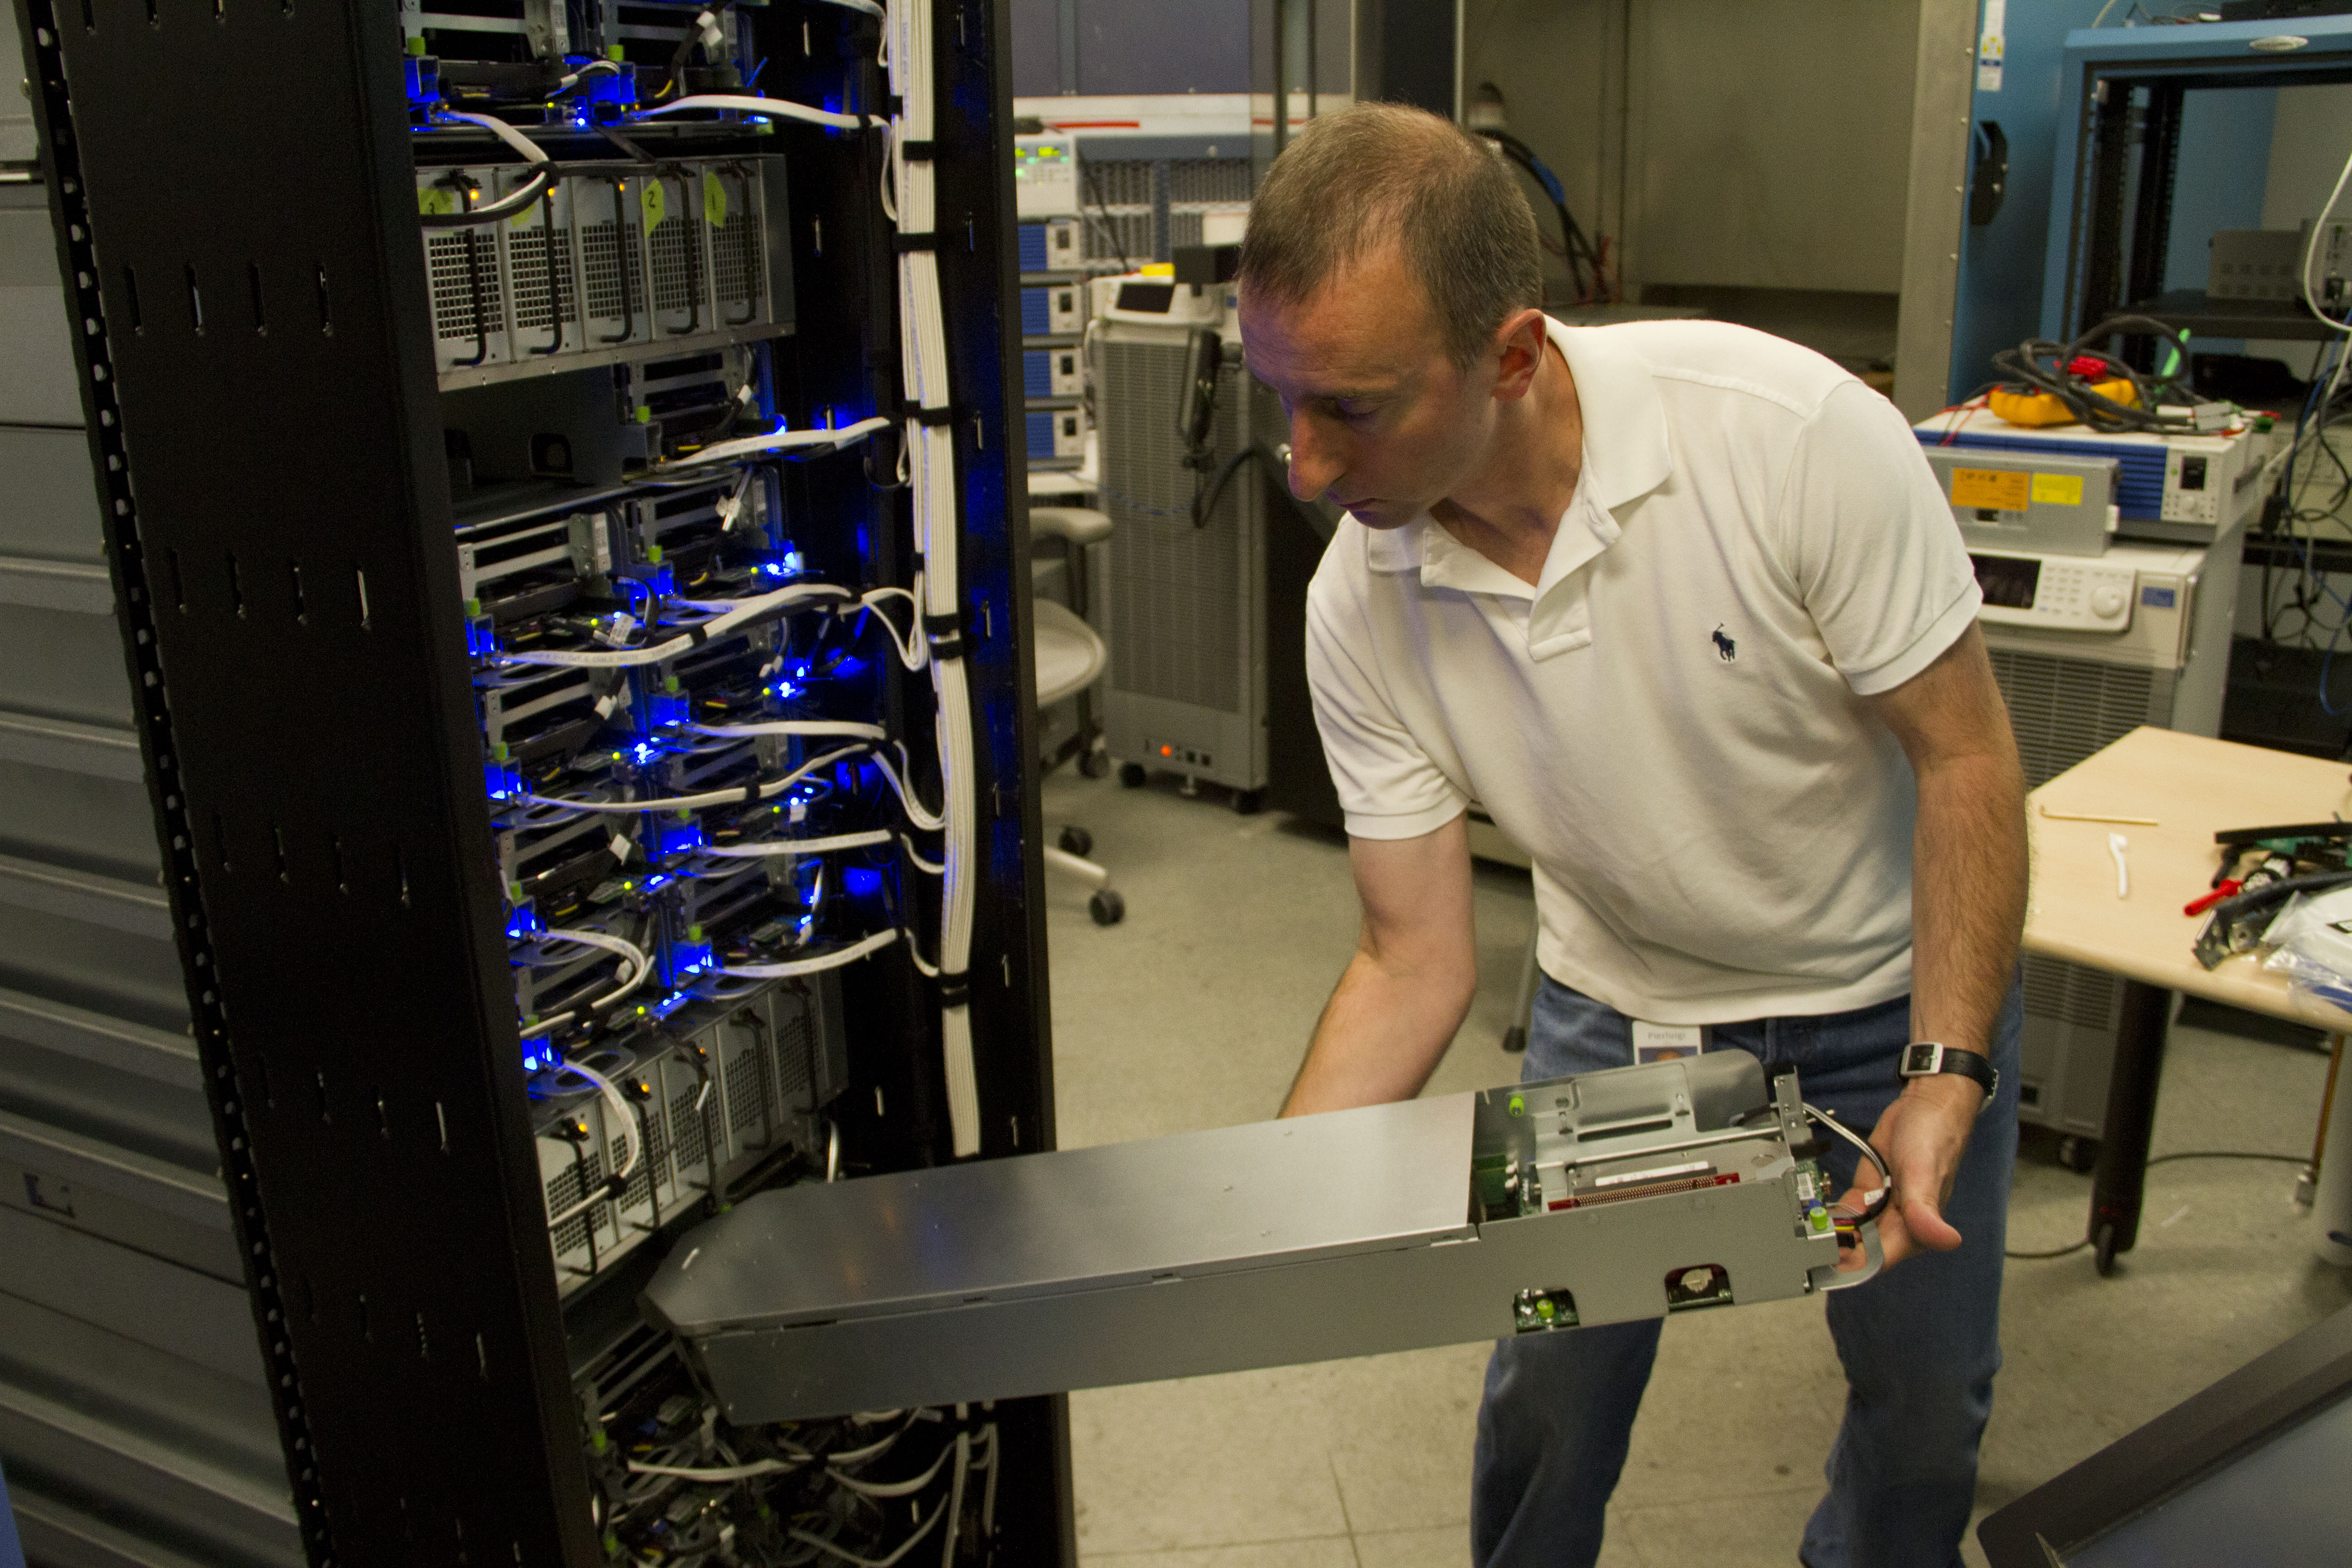
\includegraphics[width=3.5in]{../Figures/openrack2.jpg}\\[12pt]
Facebook custom-built server rack.
\end{frame}

\begin{frame}[t]{Distributed Computer (Cluster) Architecture}
\center
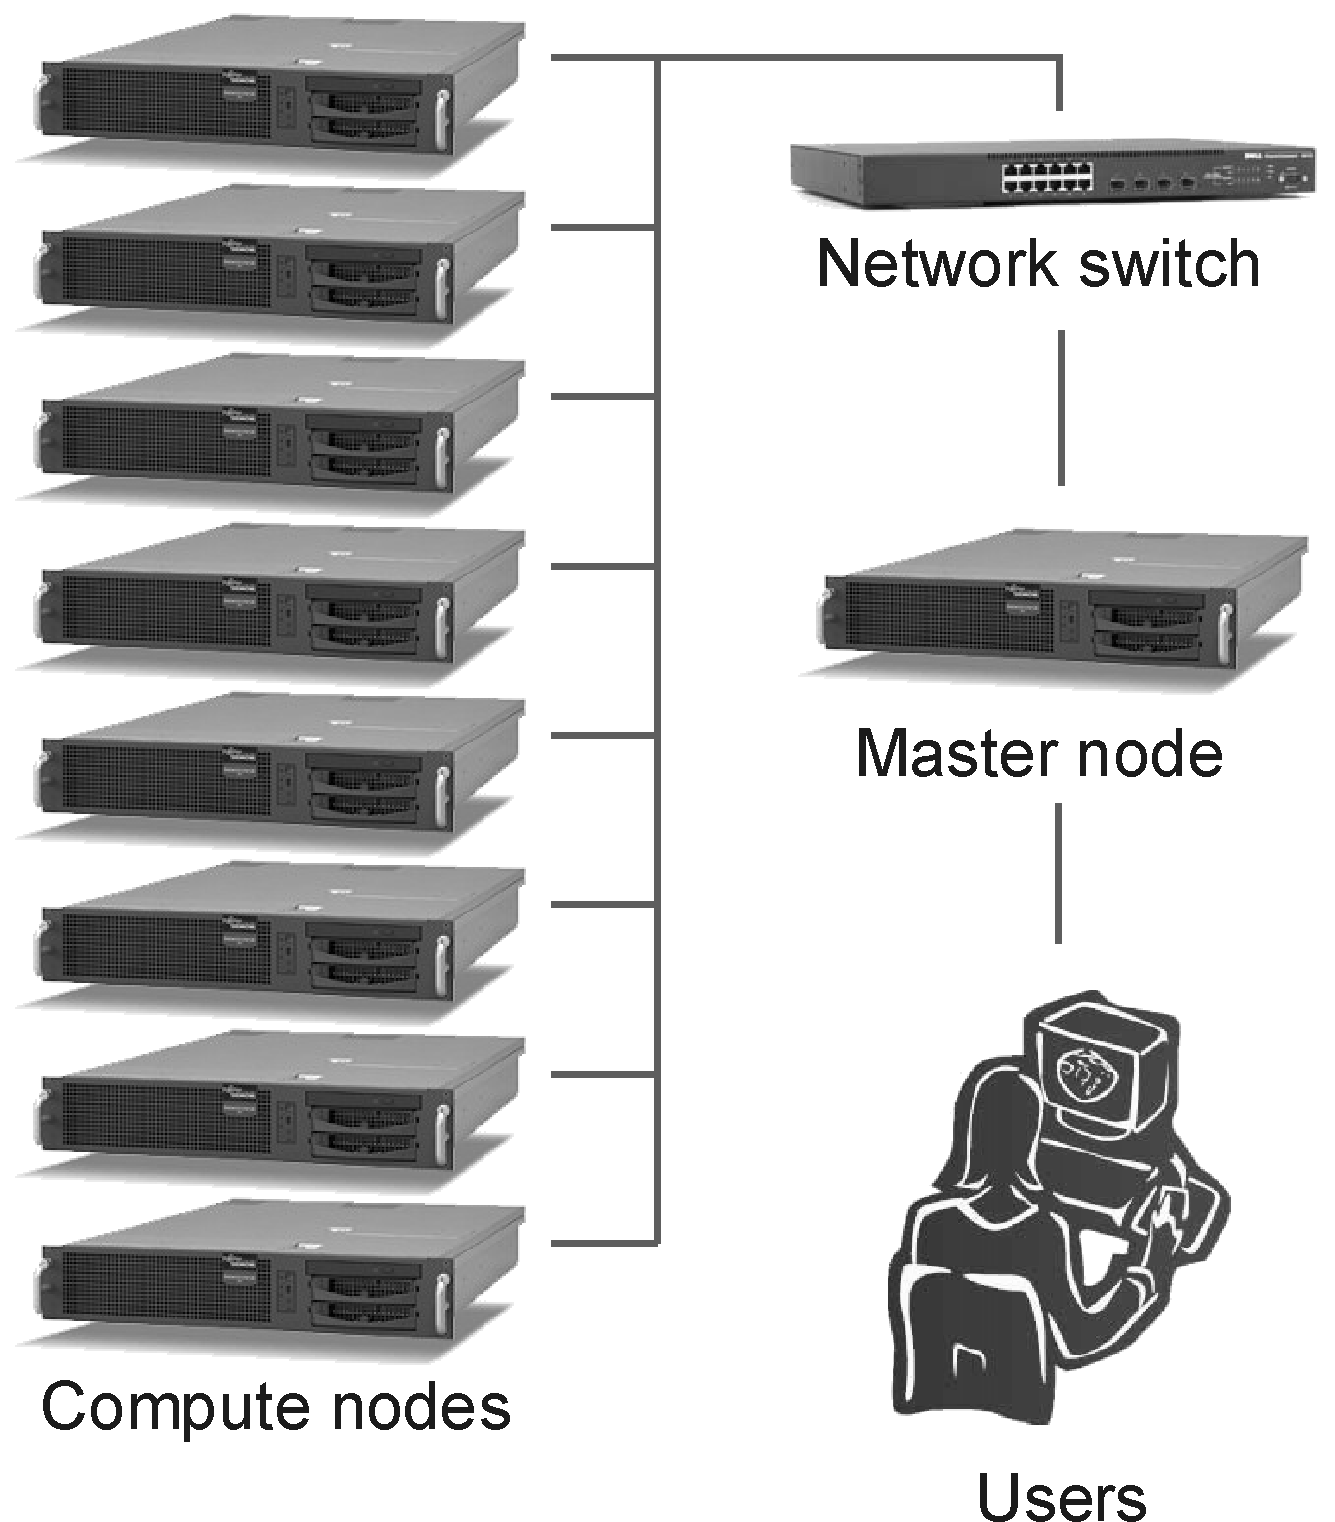
\includegraphics[height=2in]{../Figures/hpc_cluster.png}\\[12pt]
\pause \textbf{Question:} What if a one-rack cluster isn't enough?
\end{frame}


\begin{frame}[t]{Server Container}
\center
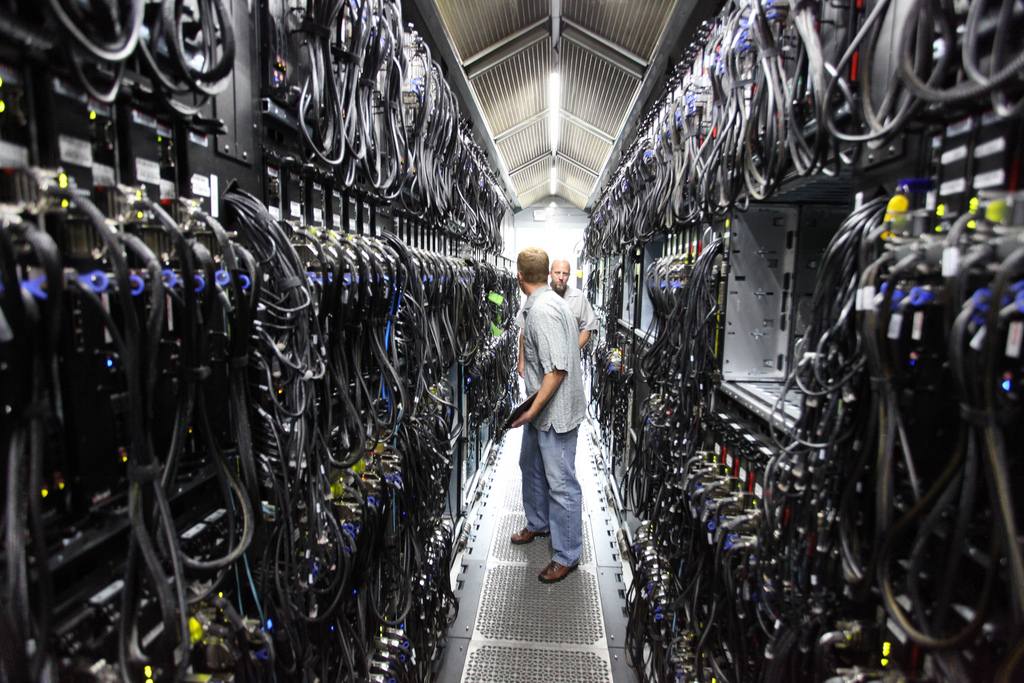
\includegraphics[width=3.5in]{../Figures/bing_container.jpg}\\
Server container used by Bing Search.\\
\pause\textbf{Question:} What if a one-container cluster isn't enough?
\end{frame}

\begin{frame}[t]{Container Hanger}
\center
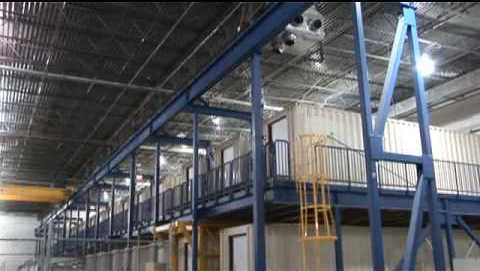
\includegraphics[width=3.5in]{../Figures/server_container.jpg}\\
Container hanger at Google data center.
{\footnotesize\url{https://www.youtube.com/watch?v=zRwPSFpLX8I}}\\
\pause\textbf{Question:} What if you don't want to manage a compute 
center?
\end{frame}

\begin{frame}[t]{Cloud Computing}
\center

\includegraphics[width=3.5in]{../Figures/clouds.png}\\[12pt]

Infrastructure as a service (IAAS) + Hardware Virtualization \\[12pt]
\url{http://aws.amazon.com/ec2/pricing/}

\end{frame}

\section{Parallel Computing Basics}
\subsection{foo}

\begin{frame}[t]{Types of Parallelism}
\begin{itemize}
\item \textbf{Shared-Memory Parallel Computing:} Running multiple threads 
concurrently with access to a single shared memory.  Low communication overhead. 
Limited scalability. Typical of multi-core 
setting.

\pause \item \textbf{Distributed Computing:} Running multiple processes on 
different machines that are networked together. High communication overhead. 
High scalability. Typical of cluster setting.
\end{itemize}
\end{frame}

\begin{frame}[t]{Types of Parallel Computing Tasks}
\begin{itemize}
\item \textbf{Embarrassingly Parallel:} Tasks need no communication between 
them at all. Near linear speedups. Examples: \pause cross validation workflows.

\pause\item \textbf{Data Parallel:} Each task performs the same operations over 
a distinct set of data elements. Tasks typically communicate only with a 
``master'' task for synchronization and not with each other. Sub-linear 
speedups. Examples: \pause data parallel 
implementations of any algorithms we've seen to date)

\pause\item \textbf{Fine-grained Parallel:} Each CPU performs local computation
but needs to frequently communicate results with other CPUs. Sub-linear 
speedups. Examples: \pause physics simulations.

\end{itemize}
\end{frame}

\begin{frame}[t]{Why the Sub-Linear Scaling?}
\begin{itemize}
\item The parallel speedup is limited by the amount of time a 
non-embarrassingly parallel process spends either in single threaded code or 
communicating with other processes.

\pause \item Amdahl's Law: Let $\alpha$ be the fraction of code that must run 
single threaded and $P$ be the number of processors. Then the maximum parallel 
speedup
is approximated by:

{\Large
$$\frac{1}{\frac{1-\alpha}{P} + \alpha}$$
}

\pause \item In the limit as $P$ goes to infinity, this ratio converges to 
$1/\alpha$.

\end{itemize}
\end{frame}

\begin{frame}[t]{Amdahl's Law}
\center
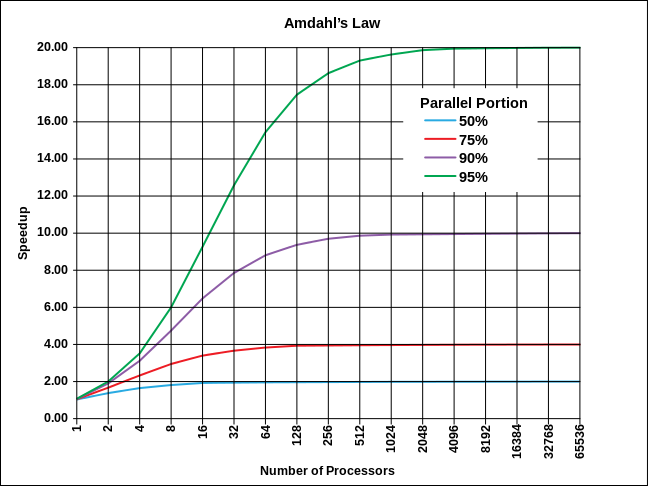
\includegraphics[width=3.5in]{../Figures/AmdahlsLaw.png}\\
\end{frame}

\section{Parallel Programming}
\subsection{foo}

\begin{frame}[t]{Imperative Programming}
\begin{itemize}
\item Imperative programming languages (C, C++, Java, etc.) have multiple 
problems with concurrency when parallelism is introduced through 
multi-threading with shared memory.

\pause \item Examples: Order-Violation, Atomicity-Violation, Deadlock, ... 

\pause \item Writing correct multi-threaded code is highly non-trivial. Since 
the order of execution of code in threads is basically random, detecting and
replicating bugs is extremely difficult.

\pause \item A key problem in PL is automatically compiling a single-threaded 
imperative program into a multi-threaded program. No such general purpose 
compiler exists today. 

\end{itemize}
\end{frame}


\begin{frame}[t]{Functional Programming}
\begin{itemize}
\item The main problems in multi-threaded imperative programs result from 
allowing mutable state through global variables accessible to all threads. 

\pause\item This is often referred to as the ``side effects'' problem. In other 
words, a function can depend on variables other than its explicit inputs, and 
modify state variables as a result of producing it's output. 

\pause \item Functional programming eliminates all of these problems by 
prohibiting mutable state variables and building computations only by nesting
function evaluations.

\pause \item There is no explicit looping, only recursion. The component 
functions are required to always return the same output when run on the same 
input.

\end{itemize}
\end{frame}


\begin{frame}[t]{Anonymous Functions}
\begin{itemize}
\item In functional programming, functions are first-class types that can be 
passed to other functions as input.

\pause\item Some mostly imperative languages like Python also support this.

\pause\item Since functional programs are often specified using many short 
functions, naming all the functions becomes tedious. 

\pause\item Anonymous functions are simply unnamed functions that can be 
written as inline expressions.

\pause\item Python supports this using the Lambda Function syntax:\\

\pause\center
{\Large \texttt{lambda x,y: x+y}}


\end{itemize}
\end{frame}

\begin{frame}[t]{Functional Programming and Parallel Computing}
\begin{itemize}
\item The advantage of functional programming is that the resulting 
programs are trivial to parallelize automatically since different arguments
to the same function can always be computed in parallel. 

\pause {\Large $$f(g(x),h(x),i(x),j(k(x),l(x)))$$}

\end{itemize}
\end{frame}

\begin{frame}[t]{Functional Programming and Data Parallel Computing}
\begin{itemize}
\item Functional programming is a natural match for data parallel computing
where we want to do things like:

\begin{itemize}
\pause \item Apply the same function to all elements in a 
data set (Map) 
\pause \item Apply a Boolean filter to select only certain data elements 
(Filter)
\pause \item Aggregate a number of data elements by summing, maxing, etc. 
(Reduce or Fold).
\end{itemize}

\pause \item It turns out that a small number of such easily parallelizable 
functional programming primitives are sufficient for creating data-parallel
implementations of machine learning algorithms. 

\end{itemize}
\end{frame}

\begin{frame}[t]{Data Parallel Computing: Map}
\begin{itemize}
\item \textbf{Map:} Applies the function $f$ to each value of the array 
$x$. This is an embarrassingly parallel operation.

$$Map(f,x)=[f(x_1),...,f(x_n)]$$

\pause
\center
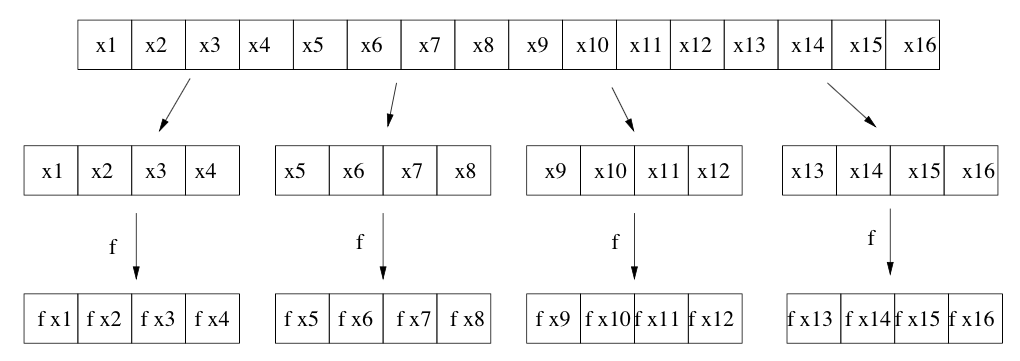
\includegraphics[width=3.5in]{../Figures/map.png}\\

\end{itemize}
\end{frame}

\begin{frame}[t]{Data Parallel Computing: Reduce}
\begin{itemize}

\item \textbf{Reduce:} Applies the function $g$ to the first two 
elements of the array $x$ recursively until the input contains a single value, 
which it then returns. 

$$Reduce(g,x) = \left\{\begin{array}{lr}
Reduce(g,[g(x_1,x_2), x_3,...,x_n]) & \mbox{ ...} n>1 \\ 
x_1 & \mbox{Otherwise} 
\end{array}\right.$$

\pause\item Ex: $Reduce(+,[3,10,20,15]) =
\pause Reduce(+,[(3+10),20,15])= 
\pause Reduce(+,[13,20,15])=
\pause Reduce(+,[(13+20),15])=
\pause Reduce(+,[33,15])=
\pause Reduce(+,[(33+15)])=
\pause 48$

\pause\item \textbf{Question:} Can we parallelize this computation?

\end{itemize}
\end{frame}


\begin{frame}[t]{Data Parallel Computing: Reduce}
\begin{itemize}

\item If the function is associative, this computation can be 
parallelized using a balanced binary tree.

\pause
{\center
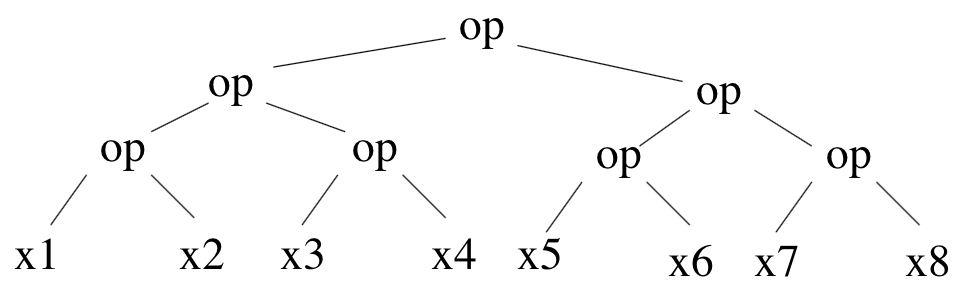
\includegraphics[width=3.5in]{../Figures/reduce.png}\\
}

\pause\item Ex: $Reduce(+,[3,10,20,15]) = 
\pause Reduce(+,[Reduce(+,[3,10]),Reduce(+,[20,15])])= 
\pause Reduce(+,[13,35])= 48$

\end{itemize}
\end{frame}




\end{document}
